\chapter{The CMS experiment in the LHC}
\chaptermark{The CMS detector in the LHC}
\label{ch:chapitre1}
\minitoc

\section{Historical background of CERN}
\label{sec:Section1}

After World War II, European physics had fallen behind.  Visionary scientists – including Pierre Auger, Niels Bohr and others – proposed creating a pan‐European laboratory to reunite researchers and share resources.  In 1949 French physicist Louis de Broglie made the first formal proposal at the Lausanne Cultural Conference.  Follow-up actions culminated in UNESCO discussions and by 1952 eleven countries had signed an agreement to form a provisional council. The name CERN (French acronym for Conseil Européen pour la Recherche Nucléaire) was then adopted.

With the organization in place, CERN quickly built its first accelerators. The Synchrocyclotron (SC) began operation in 1957 as a 600 MeV proton machine. In 1958 the SC enabled CERN’s first major discovery: the observation of a charged-pion decaying into an electron and a neutrino. Soon after, the 28 GeV Proton Synchrotron (PS) came online in 1959, briefly making CERN home to the world’s highest-energy accelerator. The PS would continue to serve as a beam source for decades to come.

\vspace{0.5 cm}

During the 1960s particle detection at CERN was dominated by the low-rate visual, bubble and spark chambers, which produced vast numbers of photographic images. This method was slow and laborious. A breakthrough came in 1968 when Georges Charpak invented the multiwire proportional chamber, a gas-filled detector with many parallel wires each connected to amplifiers. Charpak’s chamber could count particles roughly 1,000 times faster than previous techniques, ushering in the modern electronic era of particle detectors.

\vspace{0.5 cm}

CERN next pioneered colliding-beam accelerators. In 1971 the Intersecting Storage Rings (ISR) began operation, creating the world’s first high-energy proton–proton collisions. The ISR missed the 1974 'November revolution' and also the bottom quark discovery in 1977 because of an initial lack of low-mass triggers, slow DAQ, and insufficient acceptance. However, its legacy enabled the next generation collider experiments: proton stacking, space charge compensation, beam diagnostics, stochastic cooling, van-der-Meer luminosity scans, importance of efficient triggers and large angle-coverage... This success paved the way for the Super Proton Synchrotron (SPS). Approved in the early 1970s, the SPS was a 7 km circular machine straddling the Franco–Swiss border. It first circulated beam in 1976 and achieved roughly 400 GeV collision energy (above its original 300 GeV design). Later, by injecting antiprotons, CERN converted the SPS into a proton–antiproton collider. In this mode the SPS led to the 1983 discovery of the W and Z bosons, a milestone in confirming the electroweak theory (for which Carlo Rubbia and Simon van der Meer won the Nobel Prize) \cite{WandZ}.

\vspace{0.5 cm}

Building on this progress, CERN inaugurated the Large Electron–Positron collider (LEP) in 1989. LEP was a 27 km tunnel (the largest circular collider then built) designed for high-precision studies of the electroweak interaction. In its first phase it ran at about 100 GeV and produced on the order of 17 million Z bosons. LEP’s experiments performed very precise measurements; notably they confirmed that there are exactly three light neutrino species (three generations of matter particles) \cite{LEPEW2006}. After roughly eleven years of operation, LEP was shut down in 2000 to make way for the next-generation collider using the same tunnel: the Large Hadron Collider.


\section{The Large Hadron Collider}

On the September 18th 2008, the first proton beam is successfully injected within the largest particle collider ever built, namely the Large Hadron Collider (LHC). This machine and its experiments are projects of superlatives: at that time, by comparison to the Tevatron, the direct particle accelerator "competitor" based at Fermilab and in operation since 1983, the LHC had a center-of-mass energy collision seven times higher, a factor of ten in luminosity and sixteen times narrower bunch spacing; all in one ring four times larger.

Detector has been built as technological masterpieces, incorporating everything learned from previous experiments, and designed and optimised from scratch using detailed simulation. So far, their physics performance exceeds the design expectations.


The LHC \cite{EvansBryant2008}, located at CERN on the Franco-Swiss border, is the world’s largest and most powerful particle accelerator. Inaugurated in 2009, it represents the culmination of decades of progressive increases in accelerator energy at CERN. Its primary objective was the discovery of the Higgs boson — the last missing element of the Standard Model (see section XXXX) — a goal achieved in 2012 by the ATLAS \cite{ATLAS_Higgs} and CMS \cite{CMS_Higgs} collaborations. Beyond this milestone, the LHC was conceived as a versatile tool to probe particle interactions at the TeV scale, with the capability to deliver proton–proton collisions at a center-of-mass energy up to $\sqrt{s}=14$ TeV. Although this nominal value has not yet been reached, the machine currently operates at a maximum energy of 13.6 TeV. At such energies, the LHC provides a unique opportunity to test the limits of the Standard Model: both by conducting high-precision measurements that may reveal subtle deviations from theoretical predictions, and by carrying out direct searches for phenomena Beyond the Standard Model (BSM) (some of which are discussed in chapters XXXX).

\subsection{Sub-accelerator complex}
\label{subsec:SubacceleratorComplex}

Technically, the LHC functions by accelerating and colliding two counter-rotating beams of protons — or, alternatively, heavy ions — at four dedicated interaction points (IP). The ring, buried about 100 m underground, extends over a circumference of 26.66 km, composed of eight 2.45-km-long curved arcs connected by eight straight sections. Each straight section spans roughly 545 m: four of them host the major LHC experiments, while the remaining four accommodate essential machine infrastructure such as radio-frequency systems, collimators, beam dumps, and other utilities, as shown in figure \ref{fig-LHC-layout}.

\begin{figure}
    \centering
    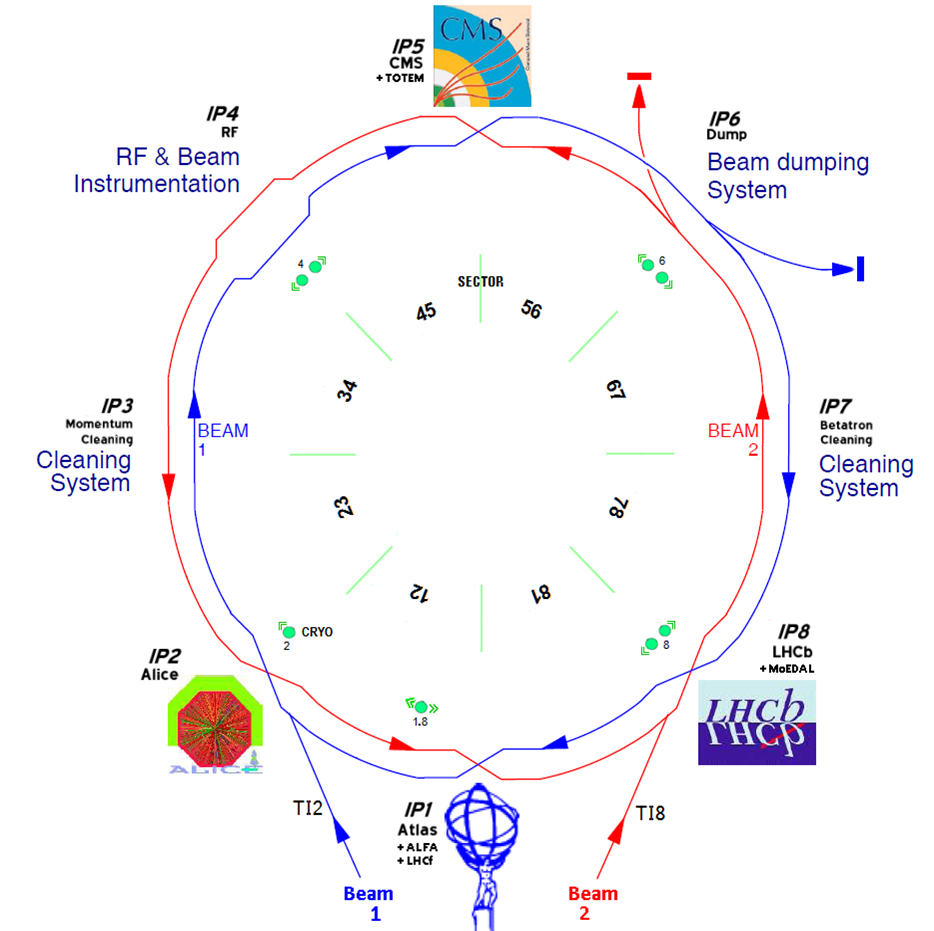
\includegraphics[width=0.6\linewidth]{Images/Ch1/LHC-layout.png}
    \caption{Illustration of the LHC geometry and experiments location.}
    \label{fig-LHC-layout}
\end{figure}

\vspace{0.5 cm}

The LHC ring is the final accelerator to a larger sub-accelerator complex. The production starts with a linear accelerator, the LINAC4, where protons are extracted from $\textrm{H}^{-}$ ions. Because of the weakly bond between the proton and two electrons, the latter can be easily stripped from the ion by going trough multiple layers of a carbon foil. At the end of this first stage, protons reach an energy of 160 MeV.

At this point, linear accelerators reach their limit, one could then consider circular collider to profit a higher center-of-mass energy collisions at the end, despite the use of a magnetic dipoles with an increasing magnetic field to confine the beam within the pipe. The beams are then injected in the Proton Synchrotron Booster (PSB), before entering the PS and latter the SPS, reaching respectively the energy of 2 GeV, 26 GeV and 450 GeV. The last step consists of preparing the two counterclockwise beams of the LHC by performing super-cycles to synchronize beam train insertion at the correct position. 

A schematic view of the CERN accelerator complex \cite{CernComplexAccelerator_ref} is shown in figure \ref{fig:CERNComplexAccelerator}.

Once in the LHC, protons are accelerated to their nominal energy (from 3.5 to 6.8 TeV, depending on the year). For that oscillating microwave fields generated by 16 superconducting radio-frequency cavities (8 per beam), housed in 4 cryo-modules, that generate a longitudinal oscillating voltage in sync with the protons that keeps them tightly bunched and accelerate them with a field of 2 MV each (5 MV/m). Each cavity is driven by a high-power klystron, a tube containing electron beams, intensity-modulated to a frequency of 400 MHz. With that protons receive 480 keV of energy per turn, or 5.3 GeV/s, during a 20-minute ramp-up period before reaching the nominal energy. 

The beams are confined in a low pressure environment, around $10^{-13}$ atm, in order to mitigate beam losses resulting from collisions between the proton beam and unknown flying objects inside the beam pipe.

In each curved arc of the LHC, a magnetic field generated individually by the 1232 superconducting NbTi dipoles bends the beams toward the center of the LHC ring. The intensity of the field goes from 0.54 to 8.33 T at the nominal as the beam accelerates. These magnets need to be cooled down to 1.9 K using super-fluid helium to let the current of 11800 A passes trough the magnet coils. So far, what limits the kinetic energy of the proton beams are the bending power of dipole magnets. To focus the beam, the LHC uses quadrupole magnets (for a total of 858) that act like magnetic lenses and focus the beam, especially at the interaction points, in order to increase luminosity. However, their focusing strength depends on the particle energy. 688 sextupole magnets are therefore used to correct this energy dependence. Finally, 168 octupole magnets introduce controlled non-linear effects that help stabilize the beam against collective instabilities (Landau damping).

Protons, as well as charged particles, emit electromagnetic radiation, known as \textit{synchroton radiation}, when they are accelerated along a curved trajectory. This energy loss per turn is scaled with the particle mass $m^{-4}$. With that electrons lose energy about $10^{13}$ times faster than protons. This is one of the main reason why protons have been chosen instead of electrons for the LHC. With a dipole field of 8.3 T, this correspond to a loss of 10 keV/turn. To compensate that, the RF cavities still operate, but to a lesser extent, under nominal conditions.

\vspace{0.5 cm}

At the nominal regime\footnote{Here for the LHC Run 3 campaign}, the LHC is circulating 2808 bunches, which are groups of about 100 billion protons (at the start). Even if the capacity of the ring is 3556 bunches, only a fraction of them are filled with protons, the beam are than organised as trains (groups of bunches) separated by empty bunches. Every bunch location is time separated from its previous by 25 ns, corresponding to the nominal LHC frequency of 40 MHz, and rotates at 11245 revolutions per second with a velocity as close as 3 m/s to the speed of light. Note that at the top energy (6.8 TeV), the stored beam energy corresponds to about 350 MJ.

Because the number of protons per bunch is decreasing after each beam crossing, the intensity of the quadrupole magnets are adjusted with time to keep the bunch squeeze enough. 

In case of beam failure, the LHC Beam Dumping System is activated to safely eject both beams into 10-meter-long graphite blocks. The beam dumping procedure is also routinely conducted at the conclusion of each LHC filing: after about eight hours, the bunches are sufficiently low in protons that they cannot be concentrated any further, and after another two to four hours, the beam is dumped.

\begin{figure}
    \centering
    \includegraphics[width=0.8\linewidth]{Images/Ch1/CERNComplexAccelerator.png}
    \caption{The CERN accelerator complex, showing the chain of accelerators leading to the LHC. The LHC is represented by the final dark blue ring, with the four major experiments indicated by yellow dots \cite{CernComplexAccelerator_ref}.}
    \label{fig:CERNComplexAccelerator}
\end{figure}


\subsection{LHC experiments}
\label{subsec:LHCExperiments}

The LHC hosts four main experiments, each designed with complementary goals and detection technologies. 

\vspace{0.5 cm}

ATLAS (\textit{A Toroidal LHC ApparatuS}) \cite{ATLAS_detector} and CMS (\textit{Compact Muon Solenoid}) \cite{CMS_detector} are the two general-purpose detectors. Despite their different designs — ATLAS being based on a large toroidal magnetic field and CMS on a high-field solenoidal magnet — they share the common mission of probing a wide range of phenomena, from Standard Model precision measurements to searches for physics Beyond the Standard Model. Both collaborations played a central role in the discovery of the Higgs boson in 2012 and continue to provide leading results in the search for new particles, such as supersymmetric states, dark matter candidates, or exotic resonances.

In contrast, LHCb (\textit{Large Hadron Collider beauty}) \cite{LHCb_detector} focuses on the study of beauty and charm hadrons. Its forward geometry and high-precision vertex detector are optimized to measure rare decays, CP violation, and flavor-changing processes, which provide an indirect window into possible new physics contributions. Thanks to its unique design, LHCb has become a world-leading experiment in the field of flavor physics, testing the consistency of the Standard Model in the quark sector with unprecedented precision.

Finally, ALICE (\textit{A Large Ion Collider Experiment}) \cite{ALICE_detector} is dedicated to the exploration of strongly interacting matter under extreme conditions. By colliding heavy ions such as lead nuclei, ALICE recreates in the laboratory the quark–gluon plasma, a state of matter believed to have existed microseconds after the Big Bang. The experiment investigates its properties—such as collective flow, particle correlations, and jet quenching—shedding light on the dynamics of the strong nuclear force in the high-density regime.

Together, these four experiments form a complementary research program: while ATLAS and CMS push the energy frontier with broad discovery potential, LHCb and ALICE exploit the LHC’s versatility to study the flavor structure of the Standard Model and the behavior of nuclear matter at extreme temperatures and densities.

\vspace{0.5 cm}

In addition to its four main experiments, the LHC hosts a set of smaller, highly specialized detectors that broaden its physics reach.

TOTEM (\textit{TOTal Elastic and diffractive cross section Measurement}, located near CMS) is devoted to measuring the total cross section of proton–proton interactions, elastic scattering, and diffraction processes. Its detectors, placed far from the interaction point in so-called “Roman pots,” are capable of detecting protons scattered at very small angles, providing insights into the strong interaction at low momentum transfer. Complementary to this, LHCf (\textit{Large Hadron Collider forward}, near ATLAS) investigates neutral particles produced at very small angles relative to the beamline. Its measurements are particularly valuable for calibrating models of cosmic-ray interactions in the atmosphere, thereby linking collider physics to astroparticle physics.

Another dedicated experiment, MoEDAL (\textit{Monopole and Exotics Detector at the LHC}, that shares the cavern at Point 8 with LHCb), is designed to search for highly ionizing particles such as magnetic monopoles or other stable, massive exotic states predicted by certain extensions of the Standard Model.

More recently, new experiments have been installed to exploit the unique forward regions of the LHC. FASER (\textit{ForwArd Search ExpeRiment}) is optimized to detect light and weakly interacting particles, such as dark photons or sterile neutrinos, which could be produced in large numbers along the beam direction but escape detection in central detectors. Similarly, SND@LHC (\textit{Scattering and Neutrino Detector at the LHC}) is the first dedicated experiment at a collider to measure neutrinos produced in high-energy proton collisions, opening a new window into both neutrino physics and forward hadronic production.

\vspace{0.5 cm}

These complementary experiments significantly enrich the LHC physics program. While the flagship detectors ATLAS, CMS, LHCb, and ALICE address broad or well-defined research domains, the smaller-scale experiments target highly specific questions, from the structure of soft QCD interactions to the search for entirely new forms of matter.


\subsection{Collisions and Luminosity}
\label{subsec:CollisionsAndLuminosity}

The following subsection describe several key parameters commonly used in particle colliders, in particular the concept of luminosity — which is directly related to the event rate — and the number of simultaneous collisions occurring within a single event. Both parameters play a crucial role in accelerator physics. Although an event is technically defined as the result of a detector readout, in our field it is often used interchangeably with the term collision.

\vspace{0.5 cm}

CMS and the LHC use \textit{instantaneous luminosity} $\mathscr{L}$ information to understand the collision environment during data-taking. The number of events $\partial N$ in a given period of time $\partial t$, knowing the process cross-section $\sigma$ is given by eq. \ref{eq:nbrEvent}:

\begin{equation}
    \frac{\partial N}{\partial t} = \mathscr{L} \cdot \sigma
    \label{eq:nbrEvent}
\end{equation}

Given the proton bunch structure of LHC beams, and assuming gaussian beam profiles colliding heads on \cite{LumiComputation}, the instantaneous luminosity is defined as eq. \ref{eq:instaneous_luminosity}: 

\begin{equation}
    \mathscr{L} = F \cdot \frac{N_p^2n_bf_{rev}\gamma}{4\pi\epsilon_n\beta^{*}}
    \label{eq:instaneous_luminosity}
\end{equation}

where:
\begin{itemize}
    \item $N_p$ is the number of particles per bunch,
    \item $n_b$ the number of bunches per beam,
    \item $f_{rev}$ the beam revolution frequency,
    \item $\gamma = 1/\sqrt{1-v^2/c^2}$ the relativistic factor (with $v$ the particle velocity and $c$ the speed of light),
    \item $\epsilon_n$ the normalized transverse emittance, that characterizes the spread of the proton distribution in the transverse plane,
    \item $\beta^{*}$ the betatron function at the IP, that characterizes the bunch envelop that oscillates around the design orbit due to the focusing provided by the magnetic field, assuming $\beta_x=\beta_y$ (the smaller the value of $\beta^{*}$, the tighter and the smaller the beam size is).
    \item $F$ is the geometric luminosity reduction factor due to the crossing angle at the IP.
\end{itemize}

The latter is defined as in eq. \ref{eq:FactorF}:

\begin{equation}
    F=\frac{1}{\sqrt{1+\left( \frac{\theta_{\textrm{IP}}\cdot\sigma_z}{2\sigma_{\textrm{IP}}} \right)^2}}
    \label{eq:FactorF}
\end{equation}

It depends on the crossing angle $\theta_\textrm{IP}$ at the IP, as well as $\sigma_z$, the RMS bunch length along the proton beam and $\sigma_{\textrm{IP}}$ the transverse RMS beam size at the IP (assuming that $\sigma_x=\sigma_y$).

Table \ref{tab:LHCnumbers} summarizes the LHC beam parameters for proton-proton collisions at nominal conditions during Run 2 \cite{LHCinfoRun2} and Run 3 \cite{LHCinfoRun3} data-taking. 

\begin{table}[]
    \centering
    \begin{tabular}{c|c|c}
        Data-taking period & 2016-2018 \cite{LHCinfoRun2} & 2022-2025 \cite{LHCinfoRun3} \\ \hline
        $N_p [\times 10^{11} \textrm{ p/bunch}]$ & 1.1-1.25 & 1.4-2.3 \\ \hline
        $n_b$                       & 2220-2556 & 2250-2736 \\ \hline
        $f_{rev}[\textrm{kHz}]$     & 11.245  & 11.245 \\ \hline
        $\epsilon_n [\mu\textrm{m}]$ & 1.8-2.2 & 3.5 \\ \hline
        $\beta^{*} [\textrm{cm}]$   & 40      & 28  \\ \hline
        Peak luminosity $(\times 10^{34} \textrm{cm}^{-2} \textrm{s}^{-1})$ & 2.1 & 3.5 \\
    \end{tabular}
    \caption{Summary of the LHC beam parameters in proton-proton collisions at nominal conditions.}
    \label{tab:LHCnumbers}
\end{table}

As discussed in \ref{subsec:SubacceleratorComplex}, since collisions occur at a 40 MHz frequency, the number of protons per bunch decreases rapidly with time, following a exponential decay: $\mathscr{L}\propto e^{-t/\tau_0}$ with $\tau_0$ of the order of 10h at the LHC today.

\vspace{0.5 cm}

Finally, the \textit{integrated luminosity} L value is used by all analysts to measure cross sections of a process being studied, or to determine the number of events expected for physics processes with well-known cross sections. L is defined as the in eq. \ref{eq:intlumi}:

\begin{equation}
    \textrm{L} = \int \mathscr{L} \, \mathrm{d}t
    \label{eq:intlumi}
\end{equation}

At the LHC, the integrated luminosity is usually defined in inverse femtobarn $\mathrm{fb}^{-1}$\footnote{$1 \, \mathrm{fb}^{-1} = 10^{-39} \, \mathrm{cm}^2$} to better compare with the magnitude of the cross sections of particle physics processes. A comparison of the integrated luminosity recorded by CMS over the years of data-taking is presented in Fig. \ref{fig:intlumi}. Summed together, the integrated luminosity from 2010 to 2025 is close to 475 $\mathrm{fb}^{-1}$.

\begin{figure}
    \centering
    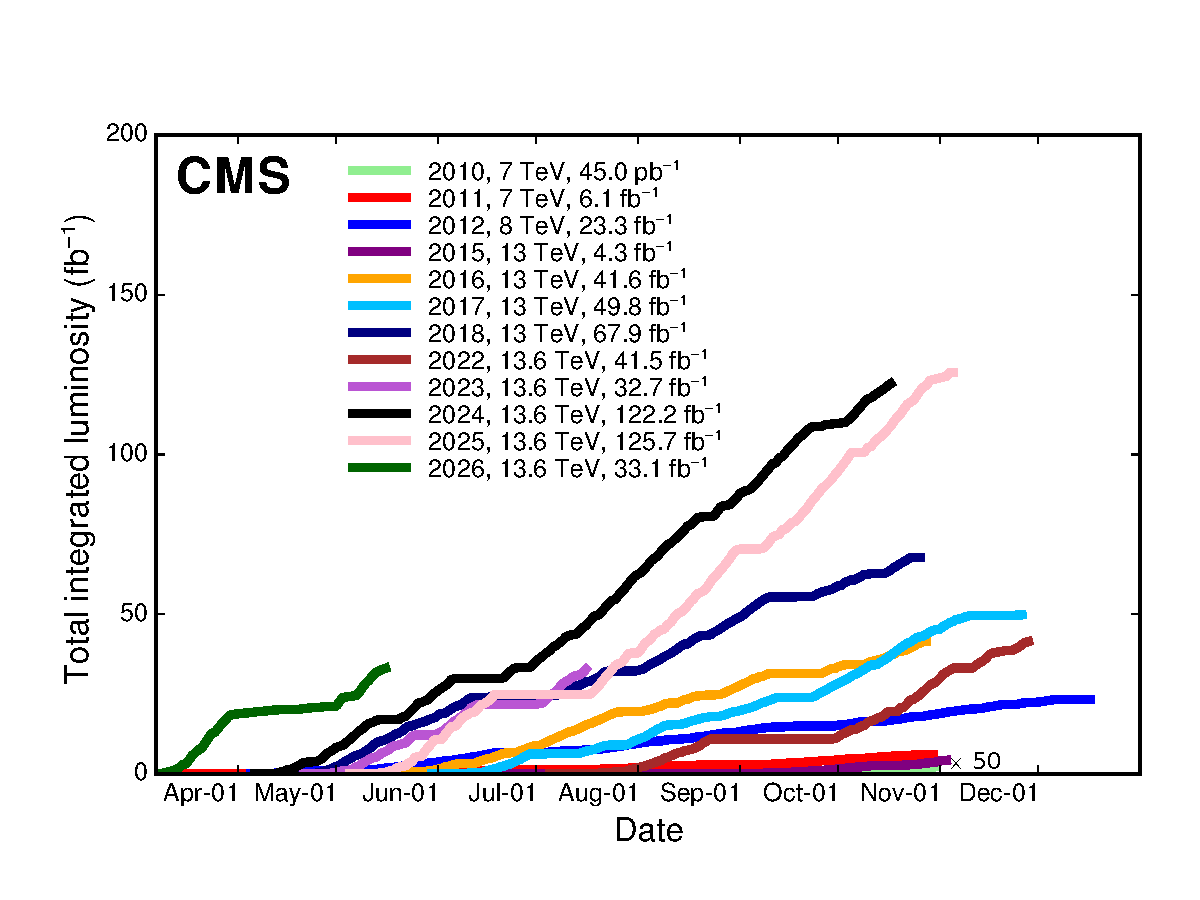
\includegraphics[width=1\linewidth]{Images/Ch1/IntLumi.pdf}
    \caption{Integrated luminosity recorded by CMS for proton-proton collisions as a function of time per year \cite{LumiIntCMS}.}
    \label{fig:intlumi}
\end{figure}

\subsection{Pile-Up}
\label{subsec:PileUp}


\begin{figure}
    \centering
    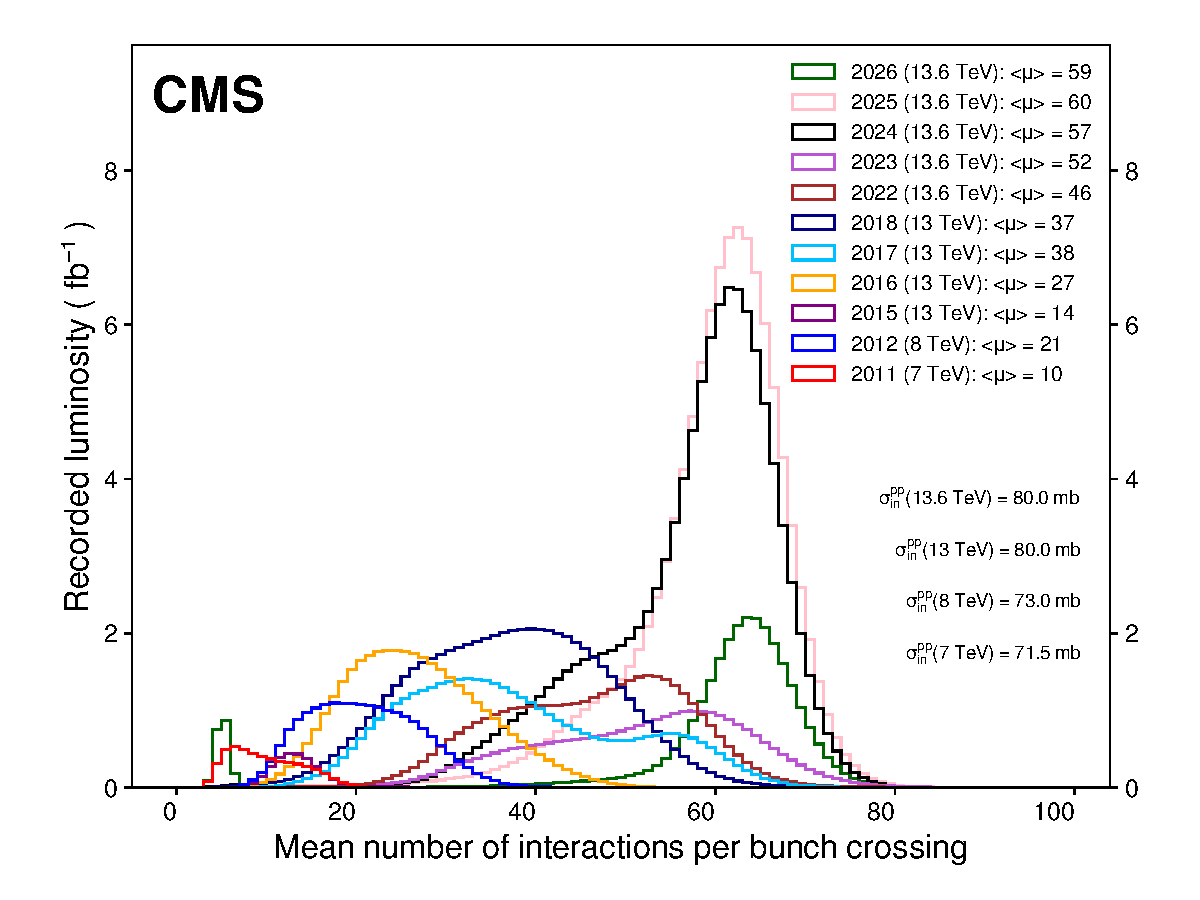
\includegraphics[width=1\linewidth]{Images/Ch1/pileup.pdf}
    \caption{Distribution of the average number of interactions per crossing (Pile-Up) for proton-proton collisions per year \cite{LumiIntCMS}.}
    \label{fig:pileup}
\end{figure}



\subsection{Schedule}

Calendrier, découvertes importantes et plans futurs 


\section{The Compact Muon Solenoid experiment}

\subsection{Coordinate system}

theta, eta, phi

\subsection{Detector dissection}

Anatomy du détecteur: détail de chaque couche (tracker, calorimetres, aimant solénoïde, chambre à muons)

\subsection{Simulations}

Des particules au détecteur (pythia, poweg, madgraph, geant4)
PU sim.
MC par année, comparaison avec d'autres exp.


\section{Event and object reconstruction at CMS}

\subsection{Trigger system}

\subsection{Identification of particles: Particle-Flow algorithm}

Système d'acquisition des données ?

Algorithme Particle-Flow ?

PU


\section{The future of the CMS detector under the HL-LHC era - Etre succinct}

\subsection{Motivations}

\subsection{Hardware change}

\subsection{Software change}

Quels parties vont êtres changés ?

Nouveautés hardware et software ?